\section{Pillar 3: Language as Learning Signal}
\label{sec:learning}

The third pillar covers signals that persist through parameter updates. We organize its methods by how much linguistic structure survives into training. Feedback-conditioned modeling retains an entire critique; self-improvement uses feedback to filter generated data; trained critics and multi-agent learning optimize the producer of feedback; process supervision localizes judgments to steps; and preference shaping compresses a judgment to one comparative bit. Richer signals preserve actionable information but require a learner capable of consuming text, while scalar compression enables mature optimization machinery at the cost of expressiveness. An orthogonal online-offline axis records whether feedback is collected from the current policy or inherited from a fixed corpus. Figure~\ref{fig:compression-spectrum} summarizes both distinctions.

\begin{figure}[!t]
    \centering
    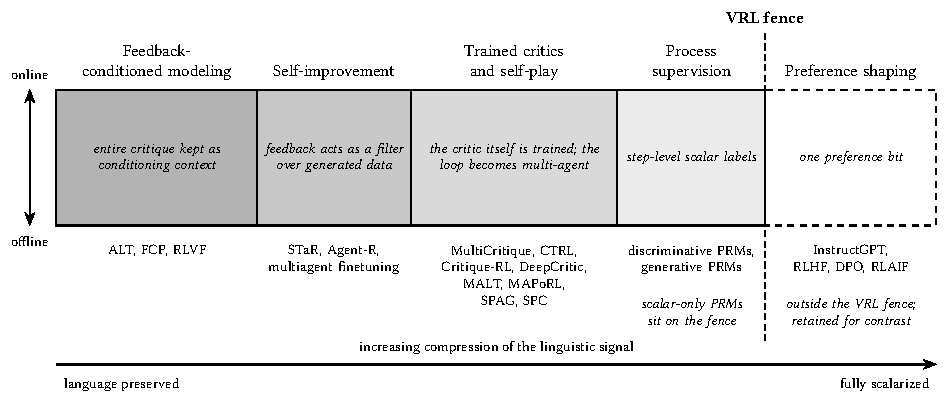
\includegraphics[width=\linewidth]{paper_images/generated/compression_spectrum.pdf}
    \Description{A horizontal spectrum orders feedback-conditioned modeling, self-improvement, trained critics and self-play, process supervision, and preference shaping by increasing compression. A vertical marker shows the VRL fence, and an orthogonal axis distinguishes online from offline feedback.}
    \caption{Training-time methods ordered by how much linguistic structure survives into the parameter update. The dashed fence places scalar-only preference optimization outside VRL and scalar-only process supervision on its boundary. Online and offline collection cut across every band.}
    \label{fig:compression-spectrum}
\end{figure}

\subsection{Feedback-Conditioned Modeling}
\label{subsec:feedback-conditioned}

At the least-compressed end, the learner receives the critique together with the response it should produce. ALT shows why retaining the critique matters, and the feedback-conditional policy formalizes training as maximum likelihood over response-feedback pairs followed by optional online bootstrapping \citep{lloret2024towards,luo2025fcp}. This family preserves corrective detail and supports targeted scope, but it also risks teaching indiscriminate compliance with inaccurate feedback.

\subsection{Self-Improvement}
\label{subsec:self-improvement}

Self-improvement uses language as a filter over model-generated trajectories. STaR retains reasoning paths that reach correct answers, while Constitutional AI filters revisions against written principles \citep{zelikman2022star,bai2022constitutional}. The approach scales cheaply because training consumes ordinary supervised examples. Its bottleneck is filter quality: when the same model generates and judges candidates, systematic errors can compound across rounds.

\subsection{Trained Critics and Critique-Based Fine-Tuning}
\label{subsec:trained-critics}

A trained critic makes feedback production an explicit capability. CTRL optimizes a critic for the downstream correction it induces, while DeepCritic combines deliberate critique with reinforcement learning over step labels \citep{xie2025teaching,yang2025deepcritic}. The design is useful when a frozen general-purpose judge limits improvement, but critic evaluation must separate helpfulness from discriminability. A critic that produces persuasive but poorly localized feedback can improve revisions while remaining an unreliable training signal.

\subsection{Multi-Agent and Self-Play Training}
\label{subsec:selfplay-training}

Jointly training feedback producers and consumers turns the loop into a multi-agent learning problem. MALT propagates outcome credit through generator, verifier, and refiner roles, while MAPoRL co-trains discussion participants for corrective and persuasive contributions \citep{motwani2024malt,park2025maporl}. Self-play can reduce external annotation, but co-adaptation creates its own instability and may reward persuasion rather than truth. The transcript's destination determines placement: context-only debate is deliberative, while transcripts or rewards that alter weights belong here.

\subsection{Process Supervision}
\label{subsec:process-supervision}

Process supervision attaches judgments to intermediate reasoning steps. Scalar click labels alone fail the linguistic-structure criterion, even when one score is provided per step. Generative process reward models remain inside the fence because language is consumed during reward computation, and free-form step critiques qualify when their content determines where credit lands \citep{lightman2024let,zhao2025genprm}. Finer granularity improves localization but raises annotation and verification cost, especially outside mathematics and code.

\subsection{Preference Shaping: The Scalar Endpoint}
\label{subsec:preference-shaping}

Preference shaping collapses a comparative judgment to one bit. InstructGPT established the reward-model plus policy-optimization recipe, and DPO trains directly from preference pairs \citep{ouyang2022training,rafailov2023direct}. These methods are retained as the compression endpoint, not as VRL proper, because the learner never consumes the rationale. Online collection can follow new policy failures; offline objectives inherit the coverage and biases of a fixed corpus.

\paragraph{Synthesis: compression versus optimizability:}
The spectrum is a conditional design rule. Preserve critiques when feedback is trustworthy and a consumer can use their structure; filter generated data when a cheap verifier exists; train critics when feedback production is the bottleneck; use process signals when localization justifies their cost; and scalarize only when throughput matters more than explanatory content. Rich feedback can improve sample efficiency, but stale offline feedback and self-generated judgments introduce coupled bias. The electronic supplement records the secondary systems, algorithmic variants, and benchmark evidence behind each band.
